\documentclass[conference, 10pt]{IEEEtran}
%\IEEEoverridecommandlockouts
% The preceding line is only needed to identify funding in the first footnote. If that is unneeded, please comment it out.
\usepackage{cite}
\usepackage{amsmath,amssymb,amsfonts}
\usepackage{algorithmic}
\usepackage{graphicx}
\usepackage{textcomp}
\usepackage{xcolor}
\usepackage[colorlinks = true,
            linkcolor = blue,
            urlcolor  = blue,
            citecolor = blue,
            anchorcolor = blue]{hyperref}
\usepackage[spanish,activeacute]{babel}

\def\BibTeX{{\rm B\kern-.05em{\sc i\kern-.025em b}\kern-.08em
    T\kern-.1667em\lower.7ex\hbox{E}\kern-.125emX}}
\begin{document}

\title{Propuesta-Proyecto Final\\Predicción del precio de bolsa de energía eléctrica del Mercado de Energía Mayorista Colombiano.}

\author{\IEEEauthorblockN{Andrea Margarita Beleño}
\IEEEauthorblockA{200620739\\
E-mail:a.beleno@uniandes.edu.co}
\and
\IEEEauthorblockN{María Valeria Gaona}
\IEEEauthorblockA{202214418\\
E-mail:mv.gaona@uniandes.edu.co}
}

\maketitle

\begin{abstract}
El precio de bolsa de energía eléctrica del Mercado Energía Mayorista (MEM) Colombiano está dado por diversos factores para generar un ambiente propicio de competencia y formación eficiente de precios, que le permitan a la demanda tener precios óptimos. Es por ello que es fundamental el análisis de este mercado para que a medida que pase el tiempo, los agentes que participan en este mercado puedan identificar factores de riesgo más rápido y así, tomar las mejores decisiones para la economía y  distribución de energía del país. El link al Github del Trabajo Final, se encuentra en el siguiente enlace:\url{https://github.com/mvgaona/Proyecto-final-MEcA-4107}\\


\end{abstract}


\section{Introducción} \label{sec:intro}
El mercado eléctrico Colombiano es un mercado competitivo en donde participan generadores, transmisores, distribuidores, consumidores y comercializadores de energía. Este mercado se divide en dos segmentos: Corto y  largo plazo, sin embargo, en el siguiente documento se presentará el análisis del mercado en corto plazo por medio de la bolsa de energía de Colombia, la cual es  administrada por XM,  en donde se presenta la participación de generadores y comercializadores de energía para la compra y venta a precio de bolsa de energía eléctrica, con el objetivo de suplir la demanda adecuada de energía en el país.   \\

De acuerdo con Trespalacios, Pantoja \& Fernández (2017)\cite{b5}, el mercado spot o la bolsa de energía hace referencia al mercado en donde se obtiene la energía eléctrica de forma instantánea, con el objetivo de lograr  un balance entre oferta y demanda. A su vez, los autores afirman que dicho precio de bolsa se define mediante un conjunto de normas que buscan precisar el nivel de referencia en caso de escasez. \\

Poveda (2012)\cite{b1} afirma que el despacho ideal es el programa de generación que está dado por el uso de los recursos más económicos hasta cubrir la demanda doméstica real, más las Transacciones Internacionales de Electricidad de Corto Plazo - TIE (exportaciones como demanda e importaciones como generación), más las pérdidas del STN (Sistema de Transmisión Nacional). Teniendo en cuenta lo anterior, el precio de bolsa está dado por el precio de oferta obtenido por medio del despacho ideal, el cual es utilizado para valorar los intercambios en bolsa.  \\
 
El correcto funcionamiento del mercado eléctrico es fundamental para el análisis de la demanda de energía en el país: si es necesario realizar estrategias en el manejo de los recursos  naturales con los que se genera energía, si la dinámica de compra y venta de energía está siendo óptima para la economía y sociedad Colombiana. Generar una proyección de estos precios permite poder hacer inferencia acerca de cómo el mercado puede estar funcionando y aunque este sea un sistema fluctuante, se puede generar predicciones acerca de su comportamiento.\\

En el siguiente documento se encuentra el análisis preliminar acerca de los datos recaudados para la predicción del precio de bolsa de energía eléctrica del mercado de energía mayorista Colombiano, en donde se implementará un modelo de Machine Learning automático en una aplicación web, que permitirá modelar futuros precios de bolsa y con ello, tomar decisiones comerciales basadas en los datos adquiridos.

\section{Problema a tratar} \label{sec:prob}
Contar con un modelo el cual prediga el precio de bolsa de energía eléctrica del MEM a partir de datos disponibles del operador del mercado, permitirá que se puedan generar decisiones con mayor conocimiento, debido a que se implementarán variables en el modelo de predicción que ayuden a tener un resultado que amortigüe la fluctuación del mercado y así, contar con un patrón de decisión más seguro ante este precio futuro.

\section{Datos} \label{sec:data}
Los datos a utilizar para el desarrollo de la predicción, se encuentran en la página del operador del mercado eléctrico colombiano XM. Esta empresa concentra todos los parámetros del sistema eléctrico colombiano que son importantes a la hora de realizar la predicción del precio de bolsa. Dentro de los predictores que de manera preliminar se consideran importantes para realizar el ejercicio (pero no se limitarán o podrán cambiarse) los siguientes:
\begin{itemize}
\item Demanda de energía nacional 
\item Precio de combustibles (utilizados para la generación de energía, como por ejemplo: carbón, gas natural, fuel oil)
\item Aportes hídricos 
\item Tipo de Generación (hidráulica, térmica, fuentes alternativas) 
\item Restricciones
\end{itemize}
De acuerdo con la operación del mercado colombiano, se tendrá en cuenta como predictor adicional, el índice interoceánico de El Niño (ONI),considerando que es un parámetro relevante para el modelo de predicción del precio de bolsa de energía eléctrica. Este parámetro se obtiene de la página web en \cite{b3}. 

\section{Métodos a implementar} \label{sec:meth}
En esta sección se realizará la descripción de la propuesta a realizar para el modelo de predicción y también para la construcción de la página web donde se visualizarán los resultados.
\subsection{Modelo propuesto} \label{sec:prop}
Debido a que el modelo del precio de bolsa es muy volátil, se dispondrá de la herramienta de árboles de decisión (Boosting trees) para realizar la predicción. Con base en los predictores mencionados en la sección \ref{sec:data}, se construirá el modelo con \textit{XG Boost} para obtener un valor predicho para el precio de bolsa de energía eléctrica en el MEM, verificando antes si existe correlación entre las variables mencionadas anteriormente. Para este método, es necesario trabajar con herramientas específicas para series de tiempo, por lo cual, se hará una búsqueda de cómo se implementan los algoritmos para este caso. \

\subsection{Página web, propuesta de visualización} \label{sec:web}
Se plantea para la visualización de datos de la predicción en la página web utilizar el paquete ``Shiny'' de R y que sea desplegado como un proyecto en Github. Inicialmente, la propuesta de visualización de la página web sería la que se muestra en la Figura ~\ref{fig1}.

\begin{figure}[htbp]
\centerline{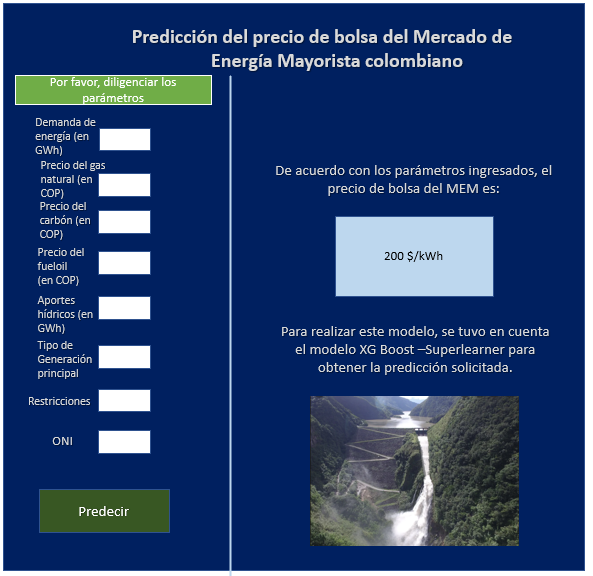
\includegraphics[width=0.3\textwidth]{../Images/Propuesta_webpage.PNG}}
\caption{Propuesta visualización página web, predicción de precio de bolsa}
\label{fig1}
\end{figure}

Se considera que la mejor forma de tener una herramienta interactiva y asequible para las personas para poder predecir el precio de bolsa, es a través de una aplicación web como la que se propone en el presente trabajo, en donde los usuarios pueden asignar valores a los predictores que influyen en el precio y así obtener un resultado de dicha predicción. Los campos en blanco son de libre diligenciamiento por el usuario y concuerdan con los predictores mencionados anteriormente. Todos los campos deben ser diligenciados. Luego se presiona el botón ``Predecir'' y en la parte derecha en el cuadro azul se visualiza el precio que se obtiene con base en esos parámetros.

\nocite{*}



\begin{thebibliography}{00}
\bibitem{b1} Poveda Núñez, M. A. (2012) “Modelamiento del precio de bolsa. Universidad Nacional de Colombia.” Bogotá D.C, Recuperado de: \url{https://repositorio.unal.edu.co/bitstream/handle/unal/21159/300038.2012.pdf?sequence=1&isAllowed=y}
\bibitem{b2} XM (2022). Sinergox de XM. Recuperado de: \url{ https://sinergox.xm.com.co/trpr/Paginas/Historicos/Historicos.aspx.} 

\bibitem{b3}Climate Prediction Center.“Cold \& Warm episodes by season” Recuperado de: \url{https://origin.cpc.ncep.noaa.gov/products/analysis_monitoring/ensostuff/ONI_v5.php}

\bibitem{b4}XGBoost time series forecast in R.“xgboost time series forecast in R” Recuperado de: \url{http://datasideoflife.com/?p=1009#:~:text=xgboost\%2C\%20or\%20Extreme\%20Gradient\%20Boosting,while\%20doing\%20time\%20series\%20predictions.}

\bibitem{b5}Trespalacios Carrasquilla, A., Pantoja Robayo, J. O., \& Fernández Taborda, Ó. A. (2017). Análisis de mercados de electricidad. EAFIT.

\end{thebibliography}


\end{document}
